\section{Experiments}
\label{sec:experiments}

For all experiments, the models were trained on the training set of MS COCO. Textual input for the {\sc Phon GRU} models was transcribed automatically using the grapheme-to-phoneme functionality with the default English voice of the eSpeak speech synthesis toolkit.\footnote{Available at \url{http://espeak.sourceforge.net}} Stress and pause markers were removed, as well as word boundaries (after storing their position for use in experiments), leaving only phoneme symbols. See Figure~\ref{fig:ipa} for an example transcription.


Visual input for all models was obtained by forwarding images through the 16-layer convolutional neural network described in \newcite{simonyan2014very} pre-trained on Imagenet \cite{ILSVRCarxiv14}, and recording the activation vectors of the pre-softmax layer. The z-score transformation was applied to these features to ease optimization. 

Most of the details of the three model types and training
hyperparameters were adopted from related work, and adapted via
informal exploration. Full exploration of the search space was not feasible due to the large number of adjustable settings in these models and their long running time. Given the importance of depth for our purposes, we did systematically explore the number of layers in the {\sc Phon GRU} and {\sc Word GRU} models. A single layer is optimal for {\sc Word GRU}. For {\sc Phon GRU}, see Section~\ref{subsec:visual} below. Other important settings were as follows:
\begin{itemize}
\setlength\itemsep{-0.5em}
\item All models: Implemented in Theano \cite{Bastien-Theano-2012}, optimized with 
  Adam \cite{DBLP:journals/corr/KingmaB14}, initial learning rate of 0.0002, minibatch size
  of 64, gradient norm clipped to 5.0.
\item {\sc Word Sum}: 1024-dimensional word embeddings, words with frequencies below 10 replaced by {\tt UNK} token.
\item {\sc Word GRU}: 1024-dimensional word embeddings, a single 1024 dimensional hidden layer, words with frequencies below 10 replaced by {\tt UNK} token.
\item {\sc Phon GRU}: 1024-dimensional hidden layers.
\end{itemize}

\subsection{Prediction of visual features}
\label{subsec:visual}
The models are trained and evaluated on the prediction of visual
feature vectors from captions. While our goal is not to develop an
image retrieval method, we use this this task as it reflects the ability to extract visually salient semantic information from language.
For the experiments on the prediction of visual features all models
were trained on the training set of MS COCO. As validation and test data we
used a random sample of 5000 images each from the MS COCO validation set. 

Figure~\ref{fig:loss} shows the value of the validation average cosine distance
between the predicted visual vector and the target vector for three
random initializations of each of the model types. 

The Phonetic GRU model is more sensitive to the initialization: one
can clearly distinguish three separate trajectories. The word-level models
are much less affected by random initialization. In terms of the
overall performance, the {\sc Phon GRU} model falls between the
{\sc Word Sum} model and the {\sc Word GRU} model.

\begin{figure}
    \centering
  \begin{minipage}{0.45\textwidth}
    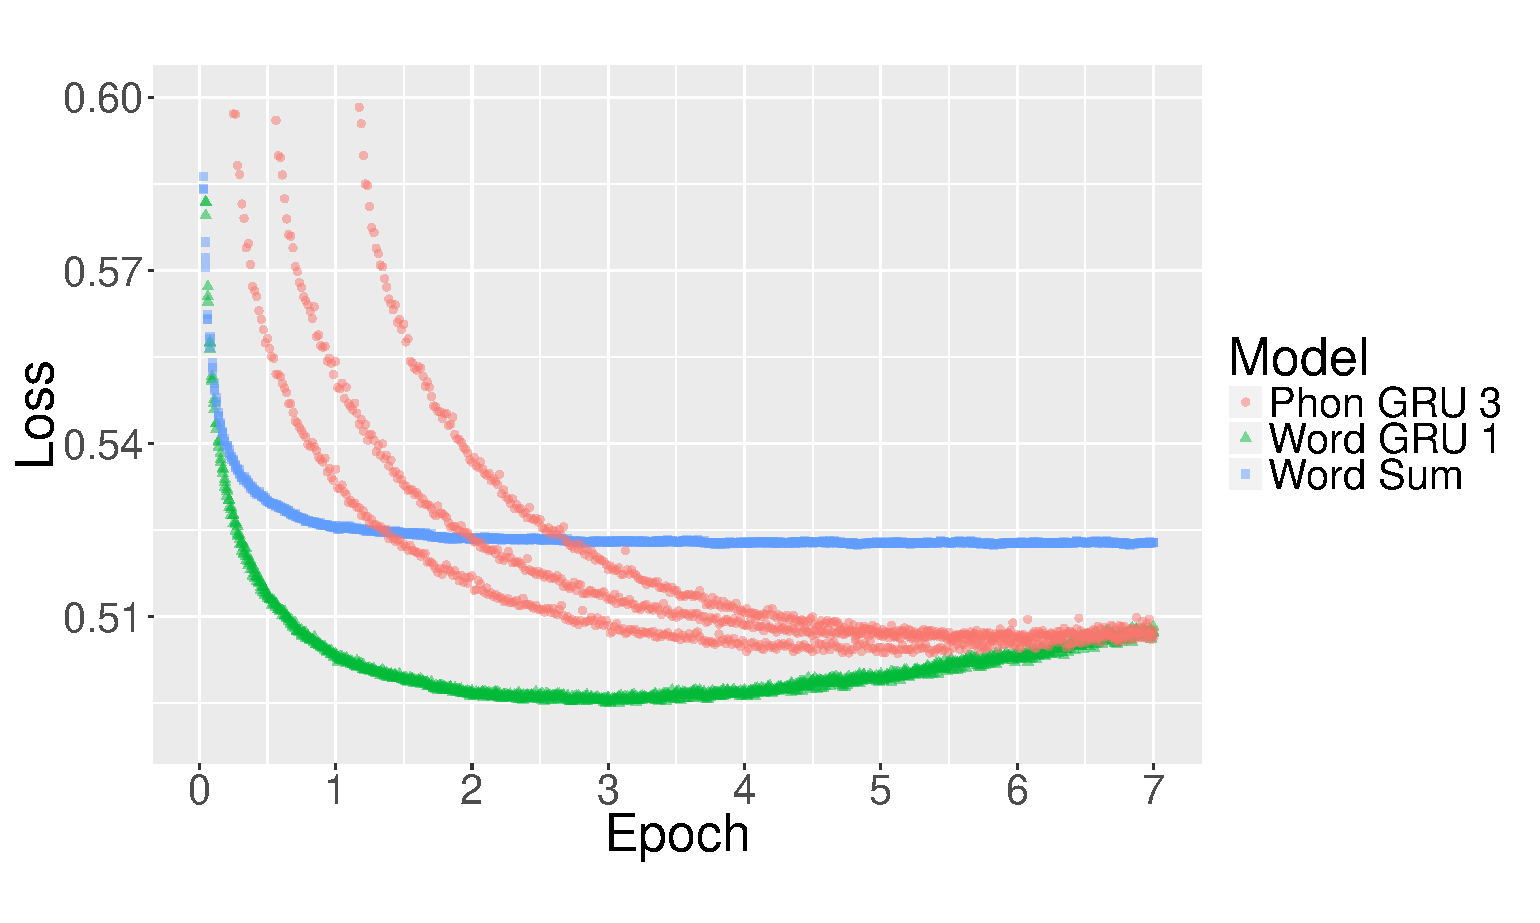
\includegraphics[scale=0.32]{loss-zoom.pdf}
    \caption{Value of the loss function on validation data during
      training. Three random initialization of each model are shown.}
    \label{fig:loss}
  \end{minipage}
\hspace{0.3cm}
  \begin{minipage}{0.45\textwidth}
    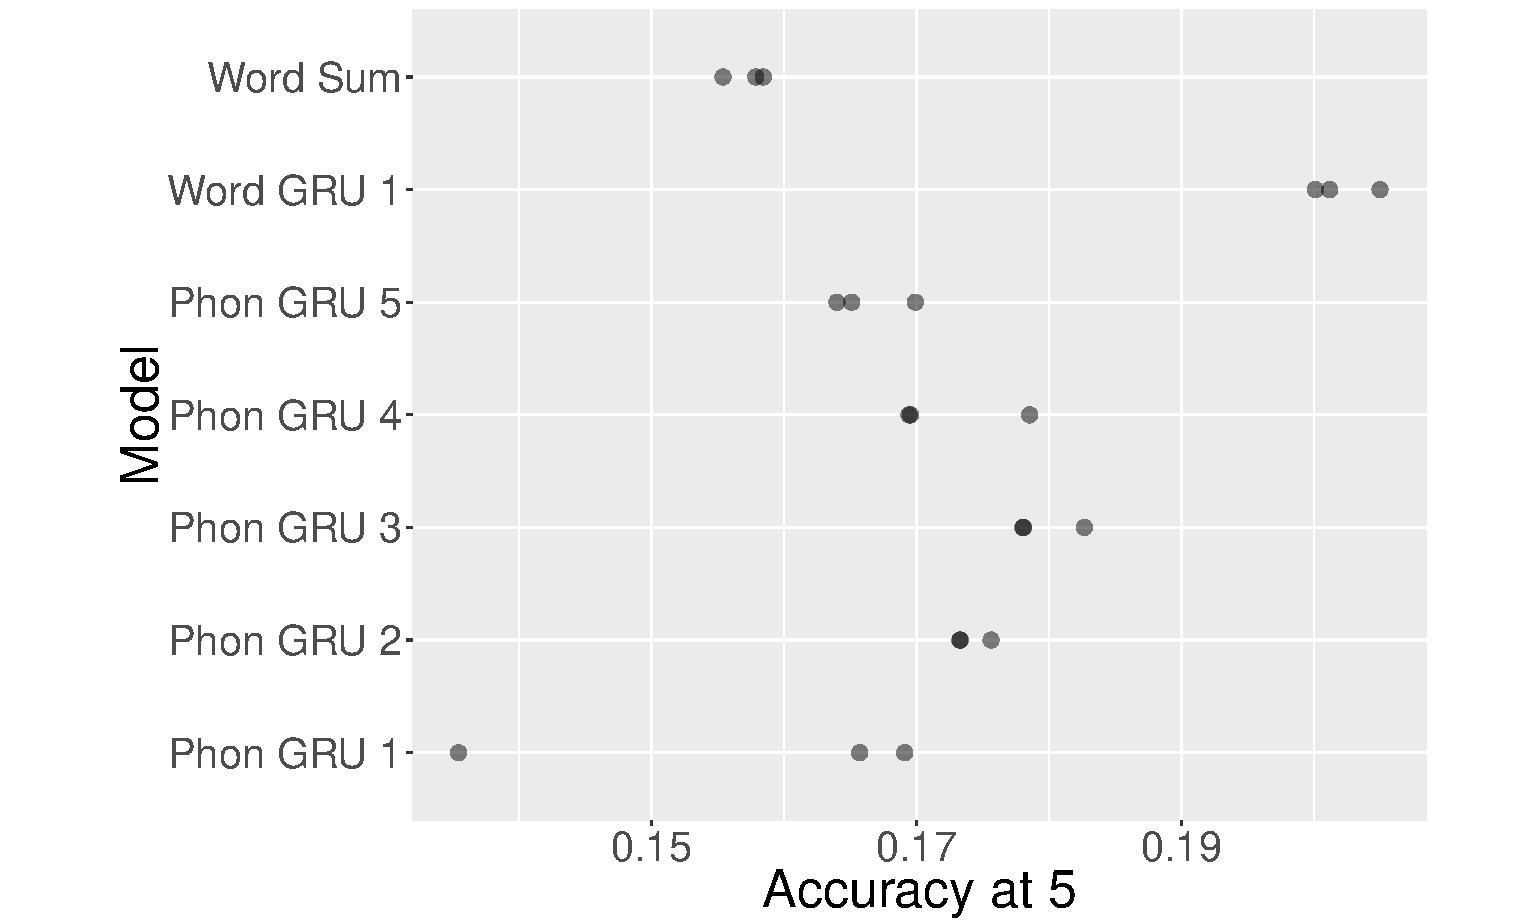
\includegraphics[scale=0.32]{accat5.pdf}
    \caption{Validation accuracy at 5 on the image retrieval task.}
    \label{fig:accat5}
  \end{minipage}
\end{figure}

We also evaluated the models on how well they perform when used to
search images: for each validation sentence the model was used to predict the
visual vector. The image vectors in the validation data were then
ranked by cosine similarity to the predicted vector, and the
proportion of times the correct image was among the top 5 was
reported. By {\it correct} image we mean the one which the sentence
was used to describe (even though often many other images are also
good matches to the sentence). 

In Figure~\ref{fig:accat5} we report the validation accuracies on this
task for the two word-level models, as well as for the Phon GRU
model with different number of hidden layers. We trained each model
version with three random initializations for each model setting, and
evaluate after each epoch. We report the score of the best epoch for
each initialization. 
The overall ranking of the models matches the direct
evaluation of the loss function above: the phoneme-level models are in
between the two word-level models. {\sc Phon GRU} with three
hidden layers is the best of the phoneme-level models.

In Table~\ref{tab:accat5test} we show the accuracies of the best
version of each of the models types on the test images; these are also
the model versions used in all subsequent experiments. The accuracy @
5 for the {\sc Word GRU} is comparable to what
\newcite{chrupala2015learning} report for their multitask {\sc
  Imaginet} model, whose visual pathway has the same
structure. \newcite{vendrov2015order} report substantially higher
scores for image search with a word level GRU model, with the
following main differences from our setting: better image features,
larger training set, and a loss function optimized for the ranking
task.\footnote{We have preliminary results indicating that most of the
  analyses in the rest of Section~\ref{sec:experiments} show the same general
  pattern for phoneme models trained following the setting of
  \newcite{vendrov2015order}.}.

% \begin{table}
%   \centering
%   \begin{tabular}{ll|r}
%  Model     & Layers & Acc. at 5 \\\hline
%  Word Sum  & 0      & 0.158 \\
%  Word GRU  & 1      & 0.205 \\\hline
%  Phon GRU  & 1      & 0.169  \\
%  Phon GRU  & 2      & 0.176  \\
%  Phon GRU  & 3      & \bf 0.183  \\  
%  Phon GRU  & 4      & 0.179 \\
%  Phon GRU  & 5      & 0.170 \\
%   \end{tabular}
% \caption{Accuracy at 5 on the image retrieval task.}
% \label{tab:accat5}
% \end{table}

\subsection{Word boundary prediction}
To explore the sensitivity of the {\sc Phon GRU} model to linguistic structure at the sub-word level, we investigated the encoding of information about word-ends in the hidden layers. Logistic regression models were trained on activation patterns of the hidden layers at all timesteps, with the objective of identifying phonemes that preceded a word boundary. For comparison, we also trained logistic regression models on \textit{n}-gram data to perform the same tasks, with positional phoneme \textit{n}-grams in the range 1-\textit{n}. The location of the word boundaries was taken from the eSpeak transcriptions, which mostly matches the location of word boundaries according to conventional English spelling. However, eSpeak models some coarticulation effects which sometimes leads to word boundaries disappearing from the transcription. For example, {\it bank of a river} is transcribed as \textipa{[baNk @v@ \*rIv@]}.
%[example of a phonetic transcription with 'ova']
All models were implemented using the {\tt LogisticRegression} implementation from Scikit-learn \cite{scikit-learn} with L2-normalization. The captions of the visual feature prediction validation data were used as training data, and those of the test set as test data. The optimal value of regularization parameter \textit{C} was determined using {\tt GridSearchCV} with 5-fold cross validation on the training set, after which the model with the optimal settings was trained on all training data.

Table~\ref{tab:boundary} reports the scores on the test set. The proportion of phonemes preceding a word boundary is 0.29, meaning that predicting {\it no word boundary} by default would be correct in 0.71 of cases. At the highest hidden layer, enough information about the word form is available for correct prediction in 0.82 of cases - substantially above the majority baseline. The lower levels allow for more accurate prediction of word boundaries: 0.86 at the middle hidden layer, and 0.88 at the bottom level.
Prediction scores of the logistic regression model based on the activation patterns of the lowest hidden layer are comparable to those of a bigram logistic regression model.

These results indicate that information on sub-word structure is only partially encoded by {\sc Phon GRU}, and is mostly absent by the time the signal from the input propagates to the top layer. The bottom layer does learn to encode a fair amount of word boundary information, but the prediction score substantially below 100\% indicates that it is rather selective. 

\begin{table}[h]
  \begin{small}
    \centering

        \begin{minipage}{0.35\textwidth}
          \centering
          \begin{tabular}{l|r}
            Model & Acc @ 5 \\\hline
            {\sc Word Sum} & 0.158 \\
            {\sc Word GRU} & 0.205 \\
            {\sc Phon GRU} & 0.180 \\
          \end{tabular}
          \caption{Image retrieval accuracy at 5 on test data for the
            versions of {\sc Word Sum}, {\sc Word GRU} and {\sc Phon
              GRU} chosen by validation.}
          \label{tab:accat5test}
        \end{minipage}
        \hspace{0.5cm}
        \begin{minipage}[r]{0.6\textwidth}
          \centering
          \begin{tabular}{lrrrr}
            \textbf{Model} & & \textbf{Acc} & \textbf{Prec} & \textbf{Rec} \\
            \hline
            Majority & & 0.71 & & \\
            \hline
            Phon GRU & Layer 1 & 0.88 & 0.82 & 0.78 \\
                           & Layer 2 & 0.86 & 0.79 & 0.71 \\
                           & Layer 3 &  0.82 & 0.74 & 0.60 \\
            \hline
            \textit{n}-gram & \textit{n} = 1 & 0.80 & 0.79 & 0.41 \\
                           & \textit{n} = 2 & 0.87 & 0.79 & 0.78 \\
                           & \textit{n} = 3 & 0.93 & 0.86 & 0.90 \\
                           & \textit{n} = 4 & 0.95 & 0.90 & 0.93
          \end{tabular}
          \caption{Prediction scores of linear regression models based
            on activation vectors of {\sc Phon GRU} and on positional
            \textit{n}-grams}
          \label{tab:boundary}
        \end{minipage}
      \end{small}

\end{table}

\subsection{Word similarity}
To understand the encoding of semantic information in {\sc Phon GRU}, we analyzed the cosine similarity of activation vectors for word pairs from the MEN dataset \cite{bruni2014multimodal}, and compared them to human similarity judgements.
For each word pair in the MEN dataset, the words were transcribed phonetically using eSpeak and then fed to {\sc Phon GRU} individually. For comparison, the words were also fed to {\sc Word GRU} and {\sc Word Sum}. Word pair similarity was quantified as the cosine similarity between the activation patterns of the hidden layers at the end-of-sentence symbol.
In contrast to {\sc Word GRU} and {\sc Word Sum}, {\sc Phon GRU} has access to the sub-word structure. To explore the role of phonemic form in word similarity, a measure of phonemic difference was included: the Levenshtein distance between the phonetic transcriptions of the two words, normalized by  the length of the longer transcription. 

Table~\ref{tab:human} shows Spearman's rank correlation coefficient between human similarity ratings from the MEN dataset and cosine similarity at the last timestep for all hidden layers. In all layers, the cosine similarities between the activation vectors for two words are significantly correlated with human similarity judgements. The strength of the correlation differs considerably between the layers, ranging from 0.09 in the first layer to 0.28 in the highest hidden layer. The second column in Table~\ref{tab:human} shows the correlations when only taking into account the 1283 word pairs of which both words appear at least 100 times in the training data. 
Correlations for both {\sc Word GRU} and {\sc Word SUM} are considerably higher than for {\sc Phon GRU}. This is expected given that these are word level models with explicit word-embeddings, while {\sc Phon GRU} builds word representations by forwarding phoneme-level input through several layers of processing.

\begin{table}[h]
  \begin{small}
    \begin{minipage}[l]{0.55\textwidth}
      \centering
      \begin{tabular}{rrr}
        & All words & Frequent words \\\hline
        {\sc Phon GRU} Layer 1 & 0.09 & 0.12\\
        Layer 2 & 0.21 & 0.33 \\
        Layer 3 & 0.28 & 0.45 \\
        \hline
        {\sc Word GRU} & 0.48 & 0.60\\	\hline
        {\sc Word Sum} & 0.42 & 0.56
      \end{tabular}
      \caption{Spearman's correlation coefficient between word-word
        cosine similarity and human similarity judgements. All
        correlations significant at \textit{p} $< 1\mathrm{e}{-4}$.
        Frequent words appear at least 100 times in the training
        data.}
      \label{tab:human}
    \end{minipage}
    \hspace{0.5cm}
    \begin{minipage}[r]{0.4\textwidth}
      \centering
      \begin{tabular}{rr}
        Layer   & $\rho$ \\\hline
        1 & $-0.30$ \\
        2 & $-0.24$ \\
        3 & $-0.15$
      \end{tabular}
      \caption{Spearman's rank correlation coefficient between {\sc
          Phon GRU} cosine similarity and phoneme-level edit
        distance. All correlations significant at \textit{p}
        $< 1\mathrm{e}{-15}$.}
      \label{tab:edit}
    \end{minipage}
  \end{small}

\end{table}

Table~\ref{tab:edit} shows Spearman's rank correlation coefficient between the edit distance and the cosine similarity of activation vectors at the hidden layers of {\sc Phon GRU}.
As expected, edit distance and cosine similarity of the activation vectors are negatively correlated: words which are more similar in form are also more similar according to the model.\footnote{Note that in the MEN dataset, meaning and word form are also (weakly) correlated: human similarity judgements and edit distance are correlated at $-0.08$ ($p< 1\mathrm{e}{-5}$).}

The negative correlation between edit distances and cosine similarities is strongest at the lowest hidden layer and weakest, though still present and stronger than for human judgements, at the third hidden layer. 

The correlations of cosine similarities with edit distance on the one hand, and human similarity rating on the other hand, indicate that the different hidden layers reflect increasing levels of representation: whereas at the lowest level mostly encodes information about form, the highest layer mostly encodes semantic information.


\subsection{Position of shared substrings}
Here we quantify the time-scale at which information is retained in
the different layers of {\sc Phon GRU}. We looked at the location of
phoneme strings shared by sentences and their nearest neighbours on
validation data. 
We determined each sentences' nearest neighbour for each hidden layer in {\sc Phon GRU}. The nearest neighbour is the sentence for which the activation vector at the end of sentence symbol has the smallest cosine distance to the activation vector of the original sentence. The position of matching substrings is the average position in the original sentence of symbols in substrings that are shared by the neighbour sentences, counted from the end of the sentence. A high mean average substring position thus means that the shared substring(s) appear early in the sentence. This gives an indirect measure of the timescale at which the different layers operate. Table~\ref{tab:example-shared} shows an example.

As can be seen in Table~\ref{tab:substrings}, the average position of shared substrings in neighbour sentences is closest to the end for the first hidden layer and moves towards the beginning of the sentence for the second and third hidden layer. This indicates a difference between the layers with regards to the timescale they represent. Whereas in the lowest layer only information from the latest timesteps is present, the higher layers retain the input  signal over longer timescales.

\begin{table}[h]
  \begin{small}
    \begin{minipage}{0.6\textwidth}
      \begin{tabular}{c}
        Layer 1 \\\hline
        A metallic bench {\bf on a path in} the {\bf park} \\
        A man riding a bicycle {\bf on a path} in a {\bf park} \\\hline
        Layer 3 \\\hline
        A metallic {\bf bench} on a path in the {\bf park} \\
        A stone park {\bf bench} sitting in an empty green {\bf park}\\ \hline
      \end{tabular}
      \caption{An illustrative sentence with its nearest neighbour at
        layer 1 and layer 3. For readability, sentences are displayed
        in conventional spelling, and only highlight matching
        substrings of length $\geq3$. In reality we used phonetic
        transcriptions to compute shared substring positions, and 
        substrings of all lengths. }
      \label{tab:example-shared}
    \end{minipage}
    \hspace{0.5cm}
    \begin{minipage}{0.35\textwidth}
      \centering
      \begin{tabular}{rr}
        Layer   & Mean position \\\hline
        1 & 12.1 \\
        2 & 14.9 \\
        3 & 16.8 \\
      \end{tabular}
      \caption{Average position of symbols in shared substrings
        between nearest neighbour sentences according to {\sc Phon
          GRU} representations at the different layers. Positions are
        indexed from end of string.}
      \label{tab:substrings}
    \end{minipage}
  \end{small}

\end{table}


